\chapter{Diseño e implementación}\label{Chapter3}

El capítulo cuenta con los componentes diseñados, la descripción
detallada de cada módulo desarrollado en el trabajo. Utilizando las definiciones
y criterios descritos en capítulos anteriores se comprende el diseño final del módulo.

% \section{Estructura del Sistema}

\section{Estructura general del sistema}

  El módulo SDI implementa un transmisor, receptor o una interfaz full-duplex,
  para esto consta de los siguientes componentes:

  \begin{itemize}
      \item Bloque de protocolo: transmisor o receptor.
      \item \textit{Transceiver}.
      \item Controlador del \textit{transceiver}.
  \end{itemize}

  % \begin{figure}[htbp]
  %     \centering
  %     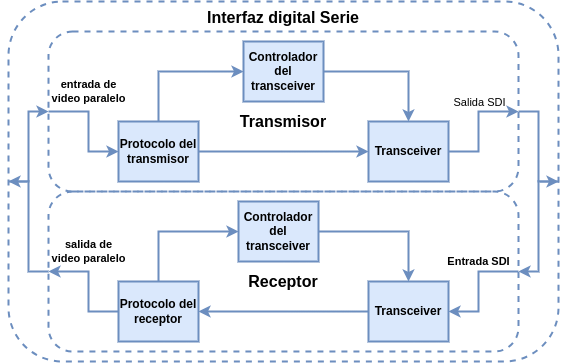
\includegraphics[width=\linewidth]{./Figures/sdi.png}
  %     \caption{Diagrama en bloques general de interfaz digital serie}\label{fig:sdi2}
  % \end{figure}

  El diseño se centró en el bloque de protocolo, ya que se supuso que se contaría con
  una FPGA que provea los otros dos, para la estructura general referirse a la
  figura~\ref{fig:sdi1}.

\subsection{Transmisor}

  El transmisor contiene los siguientes elementos:

  \begin{itemize}
      \item \textit{Scrambler} transmisor SD/HD-SDI\@.
      \item Formateador de datos HD-SDI, que incluye inserción de CRC y LN\@.
      \item \textit{Transceiver}, además de control y lógica de interfaz con el transmisor.
      \item Multiplexor de \textit{clock} de transmisor.
  \end{itemize}

  La figura~\ref{fig:sdi_tx} muestra el diagrama de bloques de nivel superior de
  la parte de protocolo, que se diseño e implementó. La figura~\ref{fig:tx_xcvr}
  muestra el diagrama de bloques de nivel superior del \textit{Transceiver}, que
  simplemente se instanció.

  % \vspace{1cm}
  \begin{figure}[htbp]
    \centering
    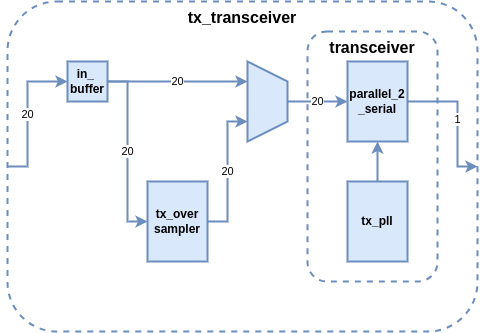
\includegraphics[width=\linewidth]{./Figures/tx_xcvr.png}
    \caption{Diagrama en bloques del transmisor de la interfaz digital serie.}\label{fig:tx_xcvr}
  \end{figure}
  % \vspace{1cm}

  % \vspace{1cm}
  \begin{figure}[htbp]
      \centering
      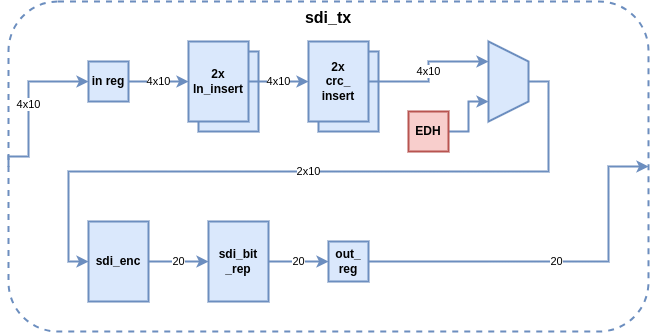
\includegraphics[width=\linewidth]{./Figures/sdi_tx.png}
      \caption{Diagrama en bloques del \textit{Transceiver} del transmisor.}\label{fig:sdi_tx}
  \end{figure}
  % \vspace{1cm}

  El transmisor realiza las siguientes funciones:
  \begin{itemize}
      % \item Inserción de LN\@.
      \item Generación e inserción de CRC y LN\@.
      \item Generación de señal de habilitación de \textit{clock}.
      \item \textit{Scrambler} y codificación NRZI (del inglés, \textit{No Return to Zero Inverted}).
      \item Cambio interno entre dos señales de \textit{clock} de referencia en el bloque transmisor.
  \end{itemize}

\subsection{Receptor}

  El receptor contiene los siguientes elementos:
  \begin{itemize}
      \item \textit{Descrambler} y alineador de palabras receptor.
      \item Extractor de CRC y LN receptor.
      \item \textit{Transceiver}, además de control y lógica de interfaz con operación de transmisor.
      \item Encuadre del receptor, con extracción de señales de temporización de video.
      \item Identificación y seguimiento de datos auxiliares.
  \end{itemize}

  La figura~\ref{fig:sdi_rx} muestra el diagrama de bloques de nivel superior de
  la parte de protocolo, que se diseño e implementó. La figura~\ref{fig:rx_xcvr}
  muestra el diagrama de bloques de nivel superior del \textit{Transceiver}, que
  simplemente se instanció.

  % \vspace{1cm}
  \begin{figure}[htbp]
      \centering
      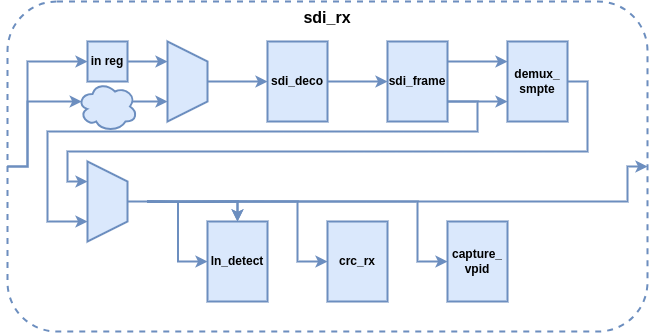
\includegraphics[width=\linewidth]{./Figures/sdi_rx.png}
      \caption{Diagrama en bloques del receptor de la interfaz digital serie.}\label{fig:sdi_rx}
  \end{figure}
  % \vspace{1cm}

  % \vspace{1cm}
  \begin{figure}[htbp]
      \centering
      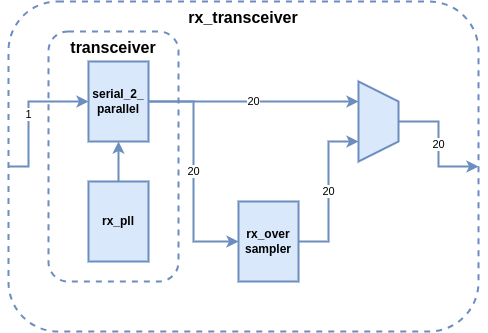
\includegraphics[width=\linewidth]{./Figures/rx_xcvr.png}
      \caption{Diagrama en bloques del \textit{Transceiver} del receptor.}\label{fig:rx_xcvr}
  \end{figure}
  % \vspace{1cm}

  El receptor realiza las siguientes funciones:
  \begin{itemize}
      \item Decodificación NRZI y \textit{Descrambler}.
      \item Alineación de palabras.
      \item Extracción de indicadores de temporización de video.
      \item Cumplimiento de cambio RP168.
      \item Extracción de LN\@.
      \item Comprobación de CRC\@.
      \item Control del \textit{transceiver}.
  \end{itemize}

\subsection{\textit{Transceivers} de Altera}

  El uso de los \textit{transceivers} de Altera, como cualquier otro fabricante,
  se da por medio de IPs que ofrecen un código encriptado y privativo y un
  archivo \textit{wrapper} que permite entender y configurar las interfaces.

  El \textit{transceivers} deserializa la entrada serie de alta velocidad. Para
  HD-SDI, la función CDR realiza la deserialización y bloquea el PLL del receptor
  a la frecuencia de los datos recibidos. Para SD-SDI, el \textit{transceivers}
  proporciona un sobremuestreo de frecuencia fija de los datos serie con el PLL
  del receptor constantemente bloqueado a un reloj de referencia, lo que permite
  al \textit{transceivers} soportar la tasa de datos de hasta 270 Mbps.
  El \textit{transceivers} puede procesar datos SD-SDI o HD-SDI\@. La tasa de datos
  puede detectarse automáticamente para que la interfaz pueda manejar ambas tasas
  de datos sin necesidad de reconfiguración del dispositivo.

  El transmisor requiere dos relojes: un reloj de datos de video paralelo (\texttt{tx\_pclk})
  y un reloj de referencia del transmisor (\texttt{tx\_serial\_refclk}). El reloj
  de video paralelo muestrea y procesa la siguiente entrada de video paralelo:
  \begin{itemize}
      \item SD-SDI\@: 27 MHz
      \item HD-SDI\@: 74,25 o 74,175 MHz
      \item 3G-SDI\@: 148,5 o 148,35 MHz
  \end{itemize}

  El \textit{transceivers} utiliza el reloj de referencia del transmisor para
  generar la salida serie de alta velocidad. Además, está configurado para
  trabajar con 20 bits, por lo que el reloj de referencia es un veinteavo de la
  tasa de datos serie. Para SD-SDI, debido a la implementación de sobremuestreo,
  la tasa de datos serie es cinco veces la tasa de bits SDI\@.
  Para operación SD-SDI, el reloj de referencia del transmisor se puede derivar
  de \texttt{pclk} usando uno de los PLLs del \textit{transceivers}. El PLL puede
  multiplicar la señal \texttt{pclk} de 27 MHz por 5/2.

  \begin{table}[h]
    \caption{Frecuencias de reloj estándar de video.}
    \centering
    \begin{tabular}{lc}
      \toprule
      \textbf{Estándar de video}  & \textbf{Frecuencia de reloj (MHz)} \\
      \midrule
      SD-SDI                      & 67,5 \\
      HD-SDI                      & 74,175 o 74,25 \\
      HD-SDI (sobremuestreo)      & 148,35 o 148,5 \\
      3G-SDI                      & 148,35 o 148,5 \\
      \bottomrule
    \end{tabular}
  \end{table}

  El \textit{transceivers} requiere un reloj de referencia para el receptor,
  \texttt{rx\_serial\_refclk}, este reloj entrena el PLL del receptor.
  Para operación SD-SDI, el reloj debe ser nominalmente 1/4 de la tasa de datos
  serie. El reloj no tiene que estar bloqueado en frecuencia a los datos.
  Para operación HD-SDI, el reloj debe ser nominalmente 1/20 de la tasa de datos
  serie. El reloj no tiene que estar bloqueado en frecuencia a los datos, porque
  el diseño solo lo utiliza para el entrenamiento del PLL del receptor.

  La interfaz del transmisor \textit{transceivers} implementa las funciones:
  \begin{itemize}
      \item Re-temporización desde el dominio del reloj de video paralelo al
      dominio del reloj del \textit{transceivers} transmisor.
      \item Sobremuestreo opcional dos veces para HD-SDI\@.
      \item Sobremuestreo del transmisor para SD-SDI\@.
  \end{itemize}

  Para lograr la funcionalidad deseada del receptor SDI, es necesario
  instanciar el controlador del \textit{transceivers}.
  Cuando la interfaz recibe SD-SDI, el PLL del receptor del \textit{transceivers}
  se bloquea al reloj de referencia del receptor.
  Cuando la interfaz recibe HD-SDI, el PLL del receptor del \textit{transceivers}
  es primero entrenado bloqueándose al reloj de referencia del receptor. Una vez
  que el PLL está bloqueado, entonces puede rastrear la tasa de datos del receptor
  actual. Si pasa un período de tiempo sin una señal SDI válida, el PLL se
  reentrena con el reloj de referencia y el proceso se repite.
  Para esto, primero, el controlador del \textit{transceivers} realiza una
  detección de tasa grosera del flujo de datos entrante. A través de la
  reconfiguración dinámica del \textit{transceivers}, luego se reprograma a la
  tasa correcta para el estándar detectado. Después de la reprogramación, el
  \textit{transceivers} intenta bloquearse al flujo entrante. Si no se ven datos
  válidos en 0,1 s, el \textit{transceivers} reinicia el receptor y realiza la
  detección de tasa nuevamente.
  Al inicio del proceso de detección de tasa, se muestrea el nivel de las tres
  señales de \textit{enable}. El nivel de estas señales y el conocimiento del
  estado actual determina si el \textit{transceivers} requiere programación. Este
  proceso asegura que el \textit{transceivers} se reprograma solo cuando es necesario.


\section{Módulos básicos}

En esta sección se presentan los módulos básicos, que son los elementos que
conectándolos entre sí permiten crear un sistema complejo y configurable.

\subsection{Replicador de bits}

  Este módulo realiza la replicación de bits de los datos entrantes, 11 veces,
  y envía 20 bits en cada ciclo de reloj. Requiere una cadencia
  alternante de 5/6/5/6 en la entrada de habilitación de reloj. La máquina
  de estados se alinea automáticamente, independientemente de si el primer
  paso de la cadencia es 5 o 6 cuando se inicia. Si la cadencia 5/6/5/6 se
  desincroniza, la máquina de estados se realineará y también activará la
  salida de error durante un ciclo de reloj.

\subsection{Insertor verificación de redundancia cíclica}

Este módulo formatea los valores CRC de 18 bits para cada canal en dos palabras
de video de 10 bits e inserta estas en los lugares apropiados inmediatamente
después de las palabras de número de línea en el EAV\@.

Un valor CRC de 18 bits se formatea en dos palabras de 10 bits que se insertan
después de las palabras EAV y número de línea. El formato de las palabras CRC
se muestra en la table~\ref{tab:crc}.

Este módulo es puramente combinacional y no contiene registros de retardo.

% \begin{center}
  \begin{table}[h]
    \centering
    \caption{Formato del CRC.}\label{tab:crc}
    \begin{tabular}{lcccccccccc}
      \toprule
      \textbf{Bit} & b9 & b8 & b7 & b6 & b5 & b4 & b3 & b2 & b1 & b0 \\
      \hline
      \textbf{CRC 0} & crc8 & crc8 & crc7 & crc6 & crc5 & crc4 & crc3 & crc2 & crc1 & crc0 \\
      \hline
      \textbf{CRC 1} & crc17 & crc16 & crc15 & crc14 & crc13 & crc12 & crc11 & crc10 & crc9 & crc8 \\
      \bottomrule
      % \hline
    \end{tabular}
  \end{table}
% \end{center}

\subsection{Codificador}

  El nivel superior del codificador HD/SD-SDI es \texttt{sdi\_enc}. Este módulo
  codifica 20 bits, 10 de luma (\textit{y}) y 10 de croma (\textit{c}); para SD,
  solo codifica el canal \textit{y}. El módulo tiene una latencia de dos ciclos
  de reloj.

  Este módulo instancia el Codificador SMPTE \texttt{smpte\_encoder} y el
  Codificador NRZ a NRZI \texttt{nrz\_2\_nrzi}.

  La salida es de 20 bits, pero para SD, solo los 10 bits menos significativos
  (LSB) son válidos. El módulo utiliza un reloj de 74,25 MHz.

\subsection{Receptor verificación de redundancia cíclica}

  Este módulo calcula el valor CRC para una línea y lo compara con el valor CRC
  recibido. El módulo realiza esta operación tanto para los canales Y como para C.
  Si se detecta un error CRC, la salida correspondiente de error CRC se activa en
  alto. Esta salida permanece activada durante el tiempo de una línea de video,
  hasta que se realice la próxima verificación de CRC\@.

  Además, el módulo captura los valores del número de línea para los dos canales
  y los emite. Los valores del número de línea son válidos durante todo el tiempo
  de la línea.

\subsection{Estándar SMPTE 292M \textit{framer}}

Es una norma para la transmisión de video digital de alta definición a través
de un enlace serie. El estándar SMPTE 259M SD-SDI es una norma equivalente
para video. Este módulo realiza el formateo en los datos decodificados.

\begin{itemize}
    \item \textbf{Entrada de datos:}
    \begin{itemize}
        \item En modo HD-SDI, el puerto de entrada \texttt{data\_i} es de 20 bits.
        \item En modo SD-SDI, solo se utilizan 10 bits.
    \end{itemize}
    
    \item \textbf{Modo de \texttt{frame\_en}:}
    \begin{itemize}
        \item \texttt{frame\_en} atado alto: resincroniza en cada detección de TRS  (del inglés, \textit{Timing Reference signal}).
        \item \texttt{frame\_en} atado a \texttt{nsp}: implementa filtrado TRS sin resincronización inmediata.
        \item \texttt{frame\_en} atado bajo: desactiva la función de formateo automático.
    \end{itemize}
\end{itemize}

\subsubsection{Detector HD señal de referencia de tiempo y codificador de desplazamiento}

El detector HD TRS (del inglés, \textit{Timing Reference signal}) identifica la secuencia
TRS de 60 bits que consiste en 20 `unos' seguidos por 40 `ceros'. El detector tiene
dos niveles principales: un detector de `unos' y un detector de `ceros'.

\begin{itemize}
    \item \textbf{Detector de unos y ceros:}
    \begin{itemize}
        \item Busca 20 unos consecutivos en \texttt{hd\_in\_1}.
        \item Busca 20 ceros consecutivos en \texttt{hd\_in\_0}.
        \item Salidas almacenadas en vectores \texttt{hd\_ones\_in}, \texttt{hd\_zeros\_in}, \\
        y \texttt{hd\_zeros\_dly}.
    \end{itemize}
    
    \item \textbf{Generación de resultados:}
    \begin{itemize}
        \item Se crea \texttt{hd\_is\_trs} mediante OR entre los vectores mencionados.
        \item \texttt{hd\_trs\_detected} se activa cuando se detecta un TRS\@.
        \item \texttt{hd\_bin\_offset} se genera desde \texttt{hd\_is\_trs}.
    \end{itemize}
\end{itemize}

\subsubsection{Detector SD señal de referencia de tiempo}

El detector SD TRS encuentra preámbulos TRS de 30 bits (3ff\textsubscript{16},
000\textsubscript{16}, 000\textsubscript{16}) en
la secuencia de datos de entrada.

\begin{itemize}
    \item \textbf{Estructura del detector:}
    \begin{itemize}
        \item Utiliza una serie de compuertas AND y NOR de 10 bits para examinar cada posición posible en el vector de entrada de 39 bits.
        \item Salidas en vectores \texttt{sd\_trs1\_match}, \texttt{sd\_trs2\_match}, y \\
        \texttt{sd\_trs2\_match}.
    \end{itemize}
    
    \item \textbf{Generación de resultados:}
    \begin{itemize}
        \item AND de los vectores anteriores crea \texttt{sd\_trs\_all\_match}.
        \item Un caso basado en \texttt{sd\_trs\_all\_match} genera \texttt{sd\_offset\_bin} y activa \texttt{sd\_trs\_error} en caso de errores.
    \end{itemize}
\end{itemize}

\subsection{Inserción de números de línea}

Este módulo cambia el formato del valor de número de línea de 11 bits en dos
palabras de 10 bits y las inserta en sus posiciones adecuadas inmediatamente
después de la palabra EAV\@. El mismo valor
de número de línea se inserta en ambos canales de video.

En el estándar SMPTE 292M, los números de línea de 11 bits deben formatearse en
dos palabras de 10 bits con el siguiente formato para cada palabra, ver tabla~\ref{tab:11bits}

% \begin{center}
\begin{table}[h]
  \centering
  \caption{Formato de los 20 bits para SMPTE 292M.}\label{tab:11bits}
  \begin{tabular}{lccccccccc}
    \toprule
    \textbf{Palabra 0} & $\sim$ln6 & ln6 & ln5 & ln4 & ln3 & ln2 & ln1 & ln0 & 0 \\
    \hline
    \textbf{Palabra 1} & 1 & 0 & 0 & 0 & ln10 & ln9 & ln8 & ln7 & 0 \\
    \bottomrule
    \hline
  \end{tabular}
\end{table}
% \end{center}

Este módulo es puramente combinatorio y no tiene registros de retardo.

% \hrulefill

\subsection{Detector de líneas}

Este módulo examina un flujo de datos de alta definición (HD) y detecta el
formato de transporte. Detecta todos los estándares de vídeo actualmente
admitidos por SMPTE 292M-2006, además de los formatos de vídeo descritos en
SMPTE RP 211. El módulo también puede utilizarse con un receptor 3G-SDI\@.

Detecta el \textit{timing} de transporte y no necesariamente el formato de vídeo real.
Cuenta palabras y líneas para determinar el estándar de vídeo. No depende de la
inclusión de paquetes ANC (del inglés, \textit{Ancillary data}) que identifican el estándar de vídeo. Además, produce
un valor de número de línea que cambia en el flanco de subida del reloj después
de la palabra XYZ de la EAV, por lo que es válido para su inserción en el campo
\texttt{ln\_o} de un flujo HD-SDI\@.

Solamente requiere como entrada uno de los canales del flujo de vídeo, ya sea Y
o C y las señales decodificadas EAV y SAV (del inglés, \textit{Start of Active Video})\@.

Cuando cambie el estándar de vídeo de entrada, se deben enviar algunos fotogramas
de vídeo (determinados por MAX\_ERRCNT) antes de comenzar el proceso de
identificación y sincronizado al nuevo formato de vídeo. Esto es para evitar que los
errores por el cambio en el estándar del vídeo hagan que el módulo pierda el
sincronizado. Sin embargo, también aumenta la latencia para que el módulo se sincronice a
un nuevo estándar cuando el estándar de vídeo de entrada cambia deliberadamente.
Si alguna lógica externa a este módulo detecta un cambio deliberado
en el estándar de vídeo de entrada, puede afirmar que la entrada requiere de este
módulo durante un ciclo de reloj para forzar al módulo a comenzar inmediatamente
el proceso de identificación y sincronizado al nuevo estándar de vídeo.

El módulo genera las siguientes salidas:

\begin{itemize}
    \item \textbf{locked:} indica cuando el módulo ha bloqueado al estándar de
    vídeo entrante. Las salidas std y ln\_o solo son válidas cuando locked es 1.
    \item \textbf{std:} un código de 4 bits que indica qué formato de transporte
    se ha detectado, codificado de la siguiente manera (las tasas son tasas de
    fotogramas):
    \begin{itemize}
        \item 0000: SMPTE 260M 1035i           30 Hz
        \item 0001: SMPTE 295M 1080i           25 Hz
        \item 0010: SMPTE 274M 1080i o 1080sF  30 Hz
        \item 0011: SMPTE 274M 1080i o 1080sF  25 Hz
        \item 0100: SMPTE 274M 1080p           30 Hz   
        \item 0101: SMPTE 274M 1080p           25 Hz   
        \item 0110: SMPTE 274M 1080p           24 Hz
        \item 0111: SMPTE 296M 720p            60 Hz
        \item 1000: SMPTE 274M 1080sF          24 Hz
        \item 1001: SMPTE 296M 720p            50 Hz
        \item 1010: SMPTE 296M 720p            30 Hz
        \item 1011: SMPTE 296M 720p            25 Hz
        \item 1100: SMPTE 296M 720p            24 Hz
        \item 1101: SMPTE 296M 1080p           60 Hz    (solo 3G-SDI nivel A)
        \item 1110: SMPTE 296M 1080p           50 Hz    (solo 3G-SDI nivel B)
    \end{itemize}
    \item \textbf{ln\_o:} Un código de 11 bits de número de línea que indica el
    número de línea actual. Este código cambia en el flanco de subida del reloj
    cuando tanto xyz como EAV están afirmados.
\end{itemize}

\subsection{Demultiplexor}

Este es el demultiplexor receptor SMPTE 425M 3G-SDI para el nivel B solamente.
Este módulo toma dos flujos de 10 bits a 148,5 MHz y los convierte en dos flujos
cada uno con dos componentes de 10 bits (Y y C) a 74,25 MHz. Típicamente, los
dos flujos de entrada de 10 bits a este módulo provienen directamente de las
salidas C (\texttt{data\_y\_i}) y Y (\texttt{data\_c\_i}) de un módulo \texttt{sdi\_framer}.

El módulo también genera señales de sincronización correctas para el vídeo,
incluyendo señales TRS, XYZ, EAV y SAV, así como información del número de
línea capturada del flujo de datos.

El módulo también crea una señal de habilitación de reloj de salida, dout\_rdy,
que se activa cuando hay datos válidos en las salidas. Si la frecuencia de reloj
de entrada es de 148,5 MHz (con \textit{clock enable} siempre activo), la dout\_rdy se activará cada
dos ciclos de reloj con un ciclo de trabajo del 50 \%. Si la frecuencia de reloj
de entrada es de 297 MHz (con ce activo cada dos ciclos de reloj), entonces la
dout\_rdy se activará un ciclo de cada cuatro con un ciclo de trabajo del 25 \%.

Nota: si se utiliza la entrada \textit{clock enable} (no conectada a 1), entonces la dout\_rdy se
activará durante varios ciclos de reloj y solo cambiará cuando la entrada \textit{clock enable}
sea 1. Por lo tanto, los dispositivos aguas abajo no deben tratar dout\_rdy
como una habilitación de reloj, sino como una señal de datos lista que debe
ser calificada con la habilitación de reloj.

\subsection{Codificador}

El codificador SD/HD-SDI de nivel superior es \texttt{sdi\_enc}. Este módulo codifica
20 bits, 10 luma (y) y 10 croma (c); para SD, solo codifica el canal y. El
módulo tiene una latencia de dos ciclos de reloj.

Este módulo instancia el codificador SMPTE \texttt{smpte\_encoder} y el codificador
NRZ a NRZI \texttt{nrz\_2\_nrzi}.

La salida es de 20 bits, pero para SD, solo los 10 bits menos significativos
(LSB) son válidos. El módulo utiliza un reloj de 74,25 MHz.

\subsubsection{\textit{Scrambler} SMPTE}

Este módulo realiza los algoritmos de scrambling SMPTE en datos de 10 bits.
Está diseñado para el polinomio $z^9+z^4+1$ de los estándares SMPTE-259M
(SD-SDI) y SMPTE-292M (HD-SDI). Cuando se codifica en HD, se utilizan 2 módulos,
pero también es posible utilizar uno solo para codificar ambos canales
ejecutando el módulo al doble de velocidad. Cuando se codifica video SD, se utiliza
un solo módulo. El módulo tiene una latencia de un ciclo de reloj.

Cuando se utiliza HD, la entrada \texttt{p\_scram} del \textit{scrambler} de croma debe
estar conectada a la salida \texttt{i\_scram\_q} del \textit{scrambler} de luma y la entrada
\texttt{p\_scram} del \textit{scrambler} de luma debe estar conectada a la salida
\texttt{i\_scram} del módulo de croma. Para SD, la entrada \texttt{p\_scram} debe
estar conectada a la salida \texttt{i\_scram\_r} del mismo módulo.

\subsubsection{\textit{Scrambler} NRZ a NRZI}

Este módulo realiza la conversión de NRZ a NRZI en datos de 10 bits utilizando el
polinomio $z+1$. El módulo tiene una latencia de un ciclo de reloj.

Cuando se implementa un codificador HD-SDI, la entrada \texttt{p\_nrzi} del
convertidor de croma debe estar conectada a \texttt{data\_o[9]} del módulo de luma
y la entrada \texttt{p\_nrzi} del convertidor de luma debe estar conectada a la
salida \texttt{i\_nrzi} del convertidor de croma. Para SD, la entrada
\texttt{p\_nrzi} debe estar conectada a la salida \texttt{data\_o[9]} de sí mismo.

\subsection{Decodificador SDI}

El módulo decodificador SDI (\texttt{sdi\_deco}) admite SD y HD\@.

Este módulo sigue las normas que definen SDI (SMPTE 259M y SMPTE 292M), que
especifica que la secuencia de bits serie se codifica de dos maneras. Primero,
se utiliza un polinomio generador de $z^9+z^4+1$ para generar una secuencia de
bits NRZ\@. Luego, se emplea un polinomio generador de $z+1$ para producir la
secuencia NRZI final sin polaridad, que se transmite a través de la capa física.

El módulo decodificador, ubicado al final del enlace SDI, revierte los dos pasos
de codificación para extraer los datos originales. Primero, se utiliza el
polinomio generador $z+1$ para convertir la secuencia de bits de NRZI a NRZ\@.
Luego, se utiliza el polinomio generador $z^9+z^4+1$ para descifrar los datos.

En el HD, se decodifican 20 bits en cada ciclo de reloj. En el SD, los 10 bits
de datos SD-SDI deben colocarse en los 10 MSB del puerto \texttt{data\_i}. Se
decodifican diez bits en cada ciclo de reloj y los 10 bits decodificados se
emiten en los 10 bits MS del puerto \texttt{data\_o}.

\subsection{Inserción de paquetes de identificación}

Este módulo inserta ID de payload de video SMPTE 352M en los flujos de datos
SD-SDI, HD-SDI o 3G-SDI\@.

Para SD-SDI, acepta un flujo de datos multiplexado Y/C de 10 bits. Clock Enable
debe afirmarse 1 de cada 11 ciclos de reloj para una tasa de transmisión de 27
MHz. Para HD-SDI, acepta dos flujos de datos de 10 bits, Y y C, cada uno de
10 bits. Clock Enable debe afirmarse cada dos ciclos de reloj para una tasa de
transmisión de datos de entrada de 74,25 MHz. Para 3G-SDI nivel A, acepta dos
flujos de datos de 10 bits. Clock Enable debe afirmarse cada dos ciclos de
reloj para una tasa de transmisión de datos de entrada de 148,5 MHz.

Para 3G-SDI nivel B, acepta cuatro flujos de datos de 10 bits. Estos pueden ser
un par de enlaces dobles SMPTE 372M o pueden ser dos señales HD-SDI
independientes pero sincronizadas. La frecuencia de reloj es de 297 MHz,
Clock Enable debe afirmarse cada dos ciclos de reloj y Data In Ready se
afirma 1 de cada 4 ciclos de reloj para una tasa de transmisión de datos de
entrada de 74,25 MHz. Los datos de entrada solo se aceptan cuando ambas
señales están en alto. Debido a que \texttt{din\_rdy} también se utiliza para
multiplexar los cuatro flujos de datos a dos flujos de datos en la salida del
módulo, debe tener un ciclo de trabajo del 50 \%: alto durante dos ciclos de
reloj y bajo durante dos ciclos de reloj.

\subsection{Identificación de paquete de video}

Este módulo inserta paquetes de identificación de carga de video SMPTE 352M~\citep{st352} en
un flujo de video. El flujo puede ser tanto HD como SD, según lo indique la
señal de entrada \texttt{hd\_sd}. El módulo sobrescribirá un paquete VPID  (del inglés, \textit{Video Packet ID}) existente si la
entrada \texttt{overwrite} está activada, sino, si ya existe un paquete VPID en
el espacio HANC, no se sobrescribirá y no se insertará un nuevo paquete.

El módulo no crea las palabras de datos de usuario del paquete VPID\@. Estas se
generan externamente y entran al módulo a través de los puertos \texttt{byte1},
\texttt{byte2}, \texttt{byte3} y \texttt{byte4}. El módulo requiere un número
de línea de interfaz en su entrada. Este número de línea debe ser válido para
la nueva línea un ciclo de reloj antes del inicio del espacio HANC, es decir,
durante la segunda palabra CRC después del EAV\@.

Este módulo también puedo eliminará cualquier paquete VPID que ocurra en
cualquier otro lugar en cualquier espacio HANC\@ usando la señal
\texttt{overwrite}. Estos paquetes se marcarán como paquetes eliminados. 

% descripción y grafiquito de todos los módulos

% \subsection{Estructura Genérica de los Módulos} PASAR A APENDICE

% poner el modulito, test y toda la bola, pero de uno solo

\section{Herramientas de simulación y verificación}

\subsection{Entorno Cocotb}

  Cocotb (del inglés, \textit{COroutine based COsimulation
  TestBench}) es un entorno de \textit{TestBench} de verificación de simulación
  basado en corrutinas para verificar RTL (en inglés,
  \textit{Register Transfer Level}) descriptos en VHDL y SystemVerilog utilizando
  Python.

  \begin{figure}[h]
    \centering
    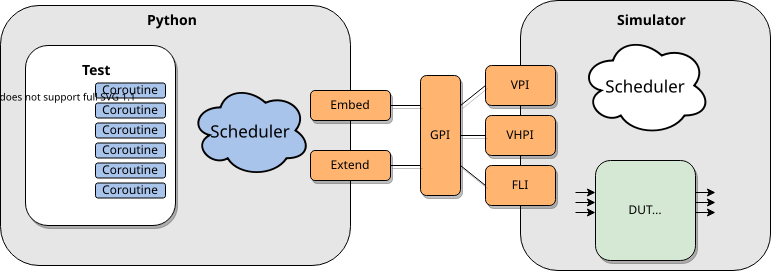
\includegraphics[width=\textwidth]{./Figures/cocotb_overview.png}
    \caption{Visión general de la conexión entre bloques y lenguajes que permite de Cocotb~\citep{cocotb}.}
  \end{figure}
  
  Cocotb fue desarrollado para hacer las pruebas más eficientes. Impulsa
  estímulos en las entradas del DUT y monitorea las salidas directamente
  desde Python, en el Apéndice~\ref{AppendixA} se puede ver un ejemplo del
  código generado para uno de los módulos desarrollados.

  Este \textit{Framework} es completamente gratuito, de código abierto (Licencia
  BSD) y alojado en GitHub. Cocotb requiere un simulador para simular el
  diseño HDL (del inglés, \textit{Hardware Description Language}) y
  se puede utilizar con una variedad de simuladores en multiples sistemas
  operativos.

  % Cocotb facilita la reutilización de código y realización de pruebas aleatorias,
  % que facilita la implementación de herramientas como UVM, sin embargo, está implementado en Python.

  Con Cocotb, los HDL tradicionales se utilizan solo para el diseño en
  sí, no para el banco de pruebas. Además, tiene soporte incorporado para
  integrarse con sistemas de integración continua y fue diseñado específicamente
  para reducir la sobrecarga de la creación de una prueba. También descubre
  automáticamente las pruebas, por lo que no se requiere un paso adicional para
  agregar una prueba a una regresión.

  La verificación se realiza integramente con Python, lo cual tiene varias
  ventajas por sobre el uso de SystemVerilog o VHDL para la verificación:

\begin{itemize}
  \item Es rápido escribir en Python, es un lenguaje muy productivo.
  \item Es fácil interfacear con otros lenguajes.
  \item Python tiene una enorme biblioteca de código existente para reutilizar.
  \item Python es interpretado: las pruebas se pueden editar y volver a ejecutar
  sin tener que recompilar el diseño.
  \item Python es popular: muchos más desarrolladores conocen Python que
  VHDL o SystemVerilog.
\end{itemize}

\subsection{Funcionamiento de Cocotb}

  Un banco de pruebas típico de Cocotb no requiere código RTL adicional.
  El Diseño Bajo Prueba o DUT (en inglés, \textit{Design-Device
  under Test}) se instancia como el \textit{toplevel} en el simulador sin ningún
  código que haga de interfaz o \textit{wrapper}.Cocotb proporciona
  estímulos a las entradas del DUT (o incluso más abajo en la jerarquía) y
  supervisa las salidas directamente desde Python.

% \begin{figure}[h]
%   \centering
%   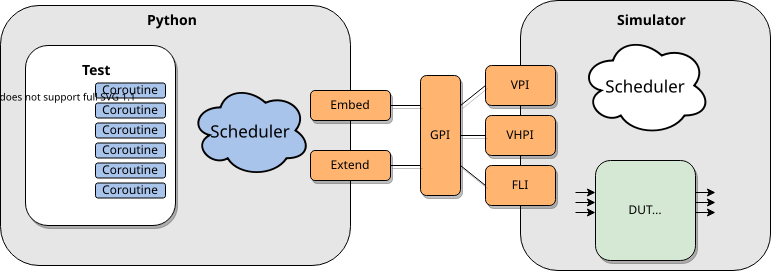
\includegraphics[width=0.7\textwidth]{./Figures/cocotb_overview.png}
%   \caption{Visión general de Cocotb.}
% \end{figure}



% \section{{Planificación}}
